\documentclass{beamer}
\usetheme{Boadilla}
\usecolortheme{beaver}

\usepackage[utf8]{inputenc}
\usepackage{ae,aecompl}
\usepackage{amsfonts}
\usepackage{mathtools}
\usepackage{listings}
\usepackage{graphicx}
\usepackage{float}

%Gör att alla slides har en frametitle, default \relax
\makeatletter
  \CheckCommand*\beamer@checkframetitle{\@ifnextchar\bgroup\beamer@inlineframetitle{}}
  \renewcommand*\beamer@checkframetitle{\global\let\beamer@frametitle\relax\@ifnextchar\bgroup\beamer@inlineframetitle{}}
\makeatother

%Gör sectionrubrik till frametitle
\addtobeamertemplate{frametitle}{\let\insertframetitle\insertsectionhead}{}

\title{Fallout: Shelter}
\subtitle{A Game Mechanics Analysis}
\author{Aron Rindstedt \and Max Block}
\date{August 12, 2015}

\begin{document}
\maketitle

\section{Introduction}
\begin{frame}
  \frametitle{Fallout: Shelter}
  \centering
  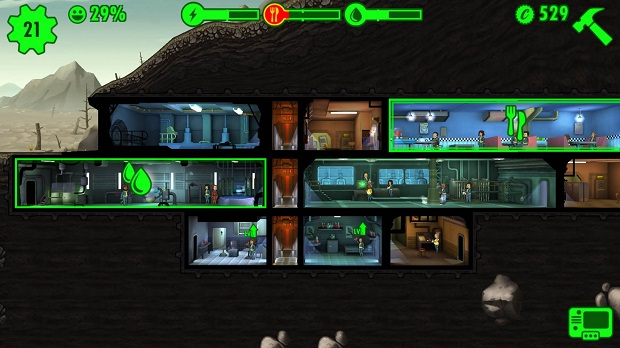
\includegraphics[scale=.3]{Fallout_Shelter_gameplay}
  \begin{itemize}
  \item Postapocalyptic mobile game
  \item You control a shelter full of dwellers
  \item One thing dwellers can do is scout
  \item Scouts retrieve bottlecaps and items
  \item Scouts face deadly challenges
  \end{itemize}
\end{frame}

\section{Character Stats}
\begin{frame}
  \begin{minipage}{.45\textwidth}
  \begin{itemize}
  \item SPECIAL stats\\($\in 1..10$ + bonus)
  \begin{itemize}
  \item Strength
  \item Perception 
  \item Endurance 
  \item Charisma 
  \item Intelligence 
  \item Agility 
  \item Luck
  \item Bonus from armour (blue)
  \end{itemize}
  \item Level (assumed to be discrete)
  \item Happiness (assumed to be insignificant)
  \item Weapon damage
  \end{itemize}
  \end{minipage}
  \hfill
  \begin{minipage}{.45\textwidth}
  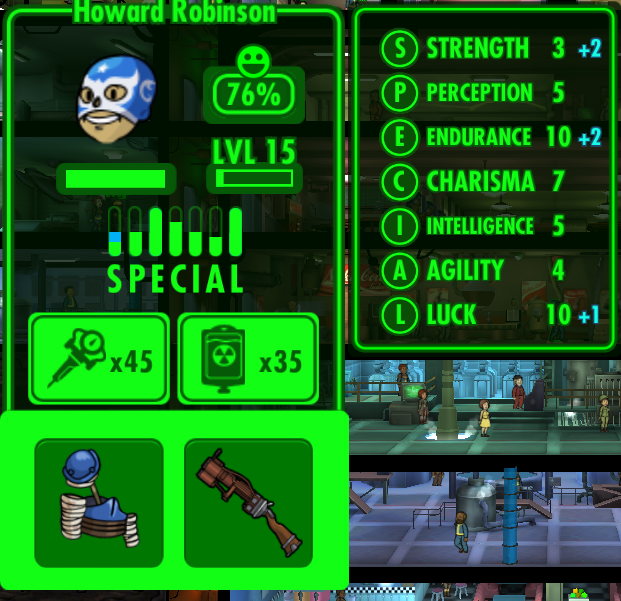
\includegraphics[width=\textwidth]{stats}
  \end{minipage}
\end{frame}


\section{Scouting}
\begin{frame}
  \begin{itemize}
  \item We wanted to know what determined how fast a scout found items and bottlecaps
  \item We performed a linear analysis and looked at the p-values
  \item The goal is to figure out if some dwellers are better scouts than others
  \end{itemize}

\end{frame}

\section{Items Per Hour}
\begin{frame}
  \frametitle{Retrieval: Items}
  \begin{table}
\caption{Number of items per hour}
\label{table:n.items}
\begin{tabular}{l|lllll}
&Estimate Std.&Error&t value&Pr(>|t|) &\\ 
\hline
(Intercept)&1.290960 &0.771921 &1.672&0.0959&.\\
level&-0.021353  & 0.017178 & -1.243 &  0.2152&  \\
dmg&-0.060882  & 0.057463 & -1.059 &  0.2906&  \\
s&-0.003986  & 0.055532 & -0.072  & 0.9428&  \\
p&-0.079242 &  0.095350 & -0.831 &  0.4069 & \\
e&0.031539 &  0.070731 &  0.446  & 0.6561&  \\
c& -0.057148  & 0.091382 & -0.625 &  0.5324&  \\
i&0.324587&0.335993&   0.966&   0.3351&  \\
a&0.214665&0.133610 &  1.607&   0.1096&  \\
l&0.042945&0.073570&0.584&0.5600&\\
\hline
\end{tabular}
\end{table}
\end{frame}

\begin{frame}
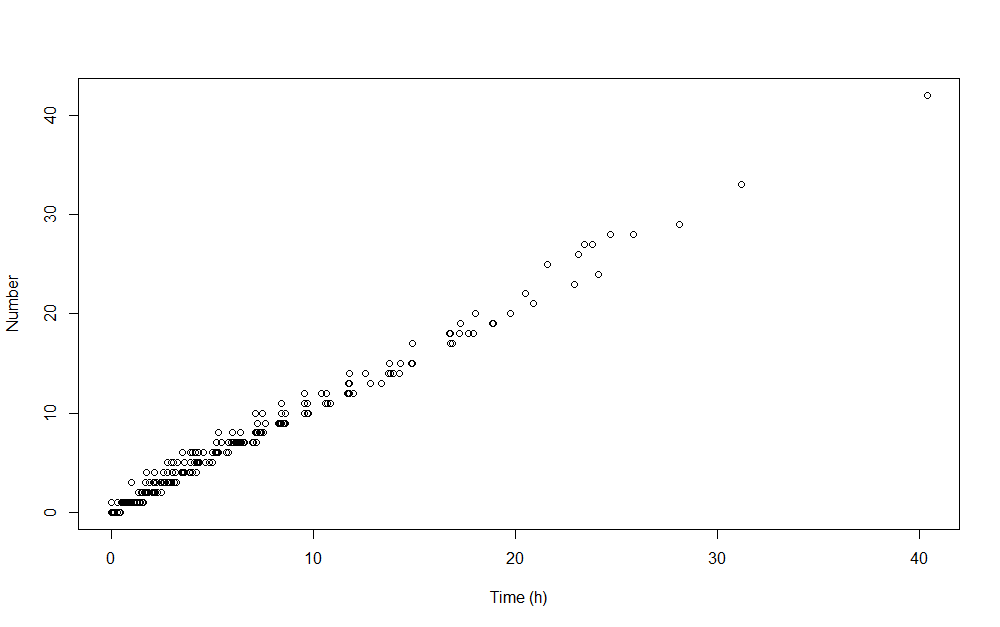
\includegraphics[width=\textwidth]{nitems.png}
\end{frame}


\section{Conclusion: Items}
\begin{frame}
  \frametitle{Retrieval: Conclusions}
  \begin{itemize}
  \item Difficult to determine what affects items found. Two p-values stand out, but are still bad.
    \begin{itemize}
    \item Intercept has p-value $0.096$
    \item Agility has p-value $0.11$
    \item<2-> Probably constant, but we need more data to be sure.
    \end{itemize}
  \end{itemize}
\end{frame}

\section{Caps Per Hour}
\begin{frame}
  \frametitle{Retrieval: Bottlecaps}
  \begin{table}
\caption{Average number of caps per hour}
\label{table:caps}
\begin{tabular}{l|lllll}
&Estimate&t value&Pr(>|t|)&\\  
\hline  
(Intercept)&83.81787937  &  11.63356 &<2e-16& ***\\
s &-0.21649106   & -0.43309 &    0.665802 &   \\
p&  0.61211724    & 0.91113 &   0.364235 &   \\
e & -0.88781188    &-1.67151 &   0.097489 &  . \\
c&-0.18453188  &  -0.31035  &  0.756888 &   \\
i& 0.19836365    & 0.35132  &  0.726024 &   \\
a  & -0.04815488  & -0.08799 &   0.930043&    \\
l &   13.48815469   & 26.55579&  <2e-16& ***\\
start.level &  -0.68088744   &  -4.25171 &   0.00004495 & *** \\ 
start.damage& -1.56703535   & -1.97083 &   0.051278 & . \\ 
level.increase & -3.44085855  & -1.97599 &   0.050683 &.  \\ 
death.damage & 0.30906873   &  0.88693  &  0.377067&\\
\hline
\end{tabular}
\end{table}
\end{frame}


\section{Conclusion: Caps}
\begin{frame}
\begin{itemize}
  \item Caps found determined by Luck (p-value < machine $\varepsilon$). There's also a base value (intercept).
  \begin{itemize}
  \item Also a small but clearly negative correlation with level, hard to tell why this is.
  \end{itemize}
  \end{itemize}
\end{frame}

\section{Survival}
\begin{frame}
  \frametitle{Survival: Intro}
  \begin{itemize}
  \item Scouts face a variety of threats.
  \item Threats can deal damage both as lost hit points and radiation, too much of either results in death.
  \item Death is nonpermanent but expensive.
  \item By calculating the expected time of death for a scout we can choose how long we dare to let our scouts roam.
  \end{itemize}
\end{frame}

\section{Summary: Survival Time}
\begin{frame}
  \frametitle{Survival: P-values}
\begin{table}[]
\centering
\caption{Survival time}
\label{table:survival.time}
\begin{tabular}{l|lll}
&Estimate Std.&Pr(>|t|)& \\ 
\hline
(Intercept)    & -0.62884167069  & 0.074911&. \\ 
s              & 0.05346141178    & 0.017339 &*\\
p              & 0.02862342249    & 0.336994 &\\
e              & 0.18123434236    & 9e-11&*** \\
c              & 0.01608604571    & 0.543637& \\
i              & 0.05055419848    & 0.052260& .\\
a              & 0.02581622298    & 0.289351& \\
l              & -0.26496311935  & 3e-7&*** \\
start.level    & 0.11302287177   & <2e-16&*** \\
start.damage   & 0.14667002834    & 7e-4&*** \\
level.increase & 0.55390718215    & 3e-8 &***\\
caps           & 0.00310366533    & 8e-8&*** \\
death.damage   & 0.01143465929    & 0.475960&\\
\hline
\end{tabular}
\end{table}
\end{frame}

\section{Survival: Tested Models}
\begin{frame}
  \frametitle{Survival: Models}
  \begin{itemize}
  \item The best p-values among the controllable variables belong to endurance, luck, level, and starting damage.
  \item Selected models
    \begin{itemize}
    \item Linear model over all four
    \item Higher order polynomial models over (exactly) one predictor
    \item Random forest
    \end{itemize}
  \end{itemize}
\end{frame}

\section{Survival: Performance}
\begin{frame}
  \begin{itemize}
  \item Since we only have limited data, error values vary, but the order is largely consistent.
  \item We used squared logarithmic errors.
    \begin{table}
      \begin{tabular}{l|ll}
        &\textbf{Model}&\textbf{MSLE}\\\hline
        1 & Linear & 0.03840157 \\
        2 & E-cubed & 0.04011285 \\
        3 & E-squared & 0.04022501 \\
        4 & L-squared & 0.04054431 \\
        5 & L-cubed & 0.0405978 \\
        6 & Level-squared & 0.0443507 \\
        7 & Level-cubed & 0.04464607 \\
        8 & Random forest & 0.07228656 \\
        \hline  &&
      \end{tabular}
  \end{table}
\end{itemize}
\end{frame}


\begin{frame}
  \begin{itemize}
  \item Linear data summary
    \begin{table}
      \centering
      \caption{Coefficients}
      \begin{tabular}{l|lllll}
        &Estimate& Std. Error& t value& Pr(>|t|)    \\
        (Intercept)  &-0.666776&   0.423767&  -1.573& 0.120256&    \\
        e            & 0.152480&   0.042116&   3.621& 0.000561& ***\\
        l            & 0.067931&   0.041358&   1.642& 0.105105&    \\
        start.level  & 0.144418&   0.009735&  14.834&  < 2e-16& ***\\
        start.damage & 0.374476&   0.056063&   6.680& 5.33e-09& ***\\
      \end{tabular}
    \end{table}
  \end{itemize}
\end{frame}


\section{Survival: Conclusions}
\begin{frame}
  \begin{itemize}
  \item A rough guess for the survival time of a given scout appears to be $(0.15(e+level)+0.4\cdot damage)$ hours.
  \item Performance varies wildly between tests, more data/more thorough analysis might be prudent.
  \end{itemize}
\end{frame}

\section{Questions}
\begin{frame}
\centering
  
  {\Huge Any questions?}


\end{frame}

\end{document}
